\batchmode
\documentclass{book}
\usepackage[letterpaper,top=2.5cm,bottom=2.5cm,left=2.5cm,right=2.5cm]{geometry}
\usepackage{makeidx}
\usepackage{natbib}
\usepackage{graphicx}
\usepackage{multicol}
\usepackage{float}
\usepackage{listings}
\usepackage{color}
\usepackage{ifthen}
\usepackage[table]{xcolor}
\usepackage{textcomp}
\usepackage{alltt}
\usepackage{ifpdf}
\ifpdf
\usepackage[pdftex,
            pagebackref=true,
            colorlinks=true,
            linkcolor=blue,
            unicode
           ]{hyperref}
\else
\usepackage[ps2pdf,
            pagebackref=true,
            colorlinks=true,
            linkcolor=blue,
            unicode
           ]{hyperref}
\usepackage{pspicture}
\fi
\usepackage[utf8]{inputenc}
\usepackage{mathptmx}
\usepackage[scaled=.90]{helvet}
\usepackage{courier}
\usepackage{sectsty}
\usepackage[titles]{tocloft}
\usepackage{doxygen}
\lstset{language=C++,inputencoding=utf8,basicstyle=\footnotesize,breaklines=true,breakatwhitespace=true,tabsize=8,numbers=left }
\usepackage{/Users/rprato/Dropbox/Programacion/Maxwell/config/latexextras}
\makeindex
\setcounter{tocdepth}{3}
\renewcommand{\footrulewidth}{0.4pt}
\renewcommand{\familydefault}{\sfdefault}
\hfuzz=15pt
\setlength{\emergencystretch}{15pt}
\hbadness=750
\tolerance=750
\begin{document}
\hypersetup{pageanchor=false,citecolor=blue}
\begin{titlepage}
\vspace*{7cm}
\begin{center}
{\Large E\-F2\-:Maxwell\-\_\-\-D\-G\-M2 \\[1ex]\large 1.\-0 }\\
\vspace*{1cm}
{\large Generated by Doxygen 1.8.0}\\
\vspace*{0.5cm}
{\small Mon Nov 12 2012 14:35:34}\\
\end{center}
\end{titlepage}
\clearemptydoublepage
\pagenumbering{roman}
\tableofcontents
\clearemptydoublepage
\pagenumbering{arabic}
\hypersetup{pageanchor=true,citecolor=blue}
\chapter{Desarrolladores E\-F2}
\label{developers}
\hypertarget{developers}{}
\hypertarget{a00001_rapt}{}\section{Ricardo Prato}\label{a00001_rapt}
\href{https://sites.google.com/site/clasesrp/}{\tt https\-://sites.\-google.\-com/site/clasesrp/} -\/\-Profesor tiempo completo -\/\-Universidad del Norte\hypertarget{a00001_cdg}{}\section{Catalina Dominguez}\label{a00001_cdg}
\href{https://sites.google.com/site/catadomingu/}{\tt https\-://sites.\-google.\-com/site/catadomingu/} -\/\-Profesora tiempo completo -\/\-Universidad del Norte 
\chapter{Class Index}
\section{Class Hierarchy}
This inheritance list is sorted roughly, but not completely, alphabetically\-:\begin{DoxyCompactList}
\item \contentsline{section}{cell}{\pageref{a00002}}{}
\item \contentsline{section}{char}{\pageref{a00003}}{}
\item \contentsline{section}{colvec}{\pageref{a00004}}{}
\item \contentsline{section}{double}{\pageref{a00005}}{}
\item \contentsline{section}{function\-\_\-handle}{\pageref{a00006}}{}
\item \contentsline{section}{handle}{\pageref{a00007}}{}
\item \contentsline{section}{integer}{\pageref{a00008}}{}
\item \contentsline{section}{logical}{\pageref{a00009}}{}
\item \contentsline{section}{matrix}{\pageref{a00010}}{}
\begin{DoxyCompactList}
\item \contentsline{section}{sparsematrix}{\pageref{a00012}}{}
\end{DoxyCompactList}
\item \contentsline{section}{rowvec}{\pageref{a00011}}{}
\item \contentsline{section}{struct}{\pageref{a00013}}{}
\item \contentsline{section}{varargin}{\pageref{a00014}}{}
\item \contentsline{section}{varargout}{\pageref{a00015}}{}
\end{DoxyCompactList}

\chapter{Class Index}
\input{annotated}
\chapter{File Index}
\section{File List}
Here is a list of all files with brief descriptions\-:\begin{DoxyCompactList}
\item\contentsline{section}{\hyperlink{a00016}{class\-\_\-substitutes.\-c} }{\pageref{a00016}}{}
\item\contentsline{section}{\hyperlink{a00017}{developers.\-c} }{\pageref{a00017}}{}
\item\contentsline{section}{\hyperlink{a00018}{dirichlet\-\_\-int.\-m} \\*Calcula la integral total de frontera para problemas no homogeneos \[ \int_{ \partial \Omega} \, n \times \curl{\bds{u}} \cdot \bds{\phi}_j \, \mathrm{d}x \] donde $ \bds{\phi}_i $ es una función base (elementos de Whitney en 2\-D) }{\pageref{a00018}}{}
\item\contentsline{section}{\hyperlink{a00019}{E\-\_\-error3.\-m} \\*Calcula el error (en caso de tener solución exacta) \[ \Vert E-E_h \Vert_{H(curl,\Omega)} \] }{\pageref{a00019}}{}
\item\contentsline{section}{\hyperlink{a00020}{Ece.\-m} \\*Calcula el valor de la función exacta (dada en rhs) en el punto xs }{\pageref{a00020}}{}
\item\contentsline{section}{\hyperlink{a00021}{Edgesnum\-\_\-\-Maxwell.\-m} \\*Inicializa la numeración de los lados de la malla provista por malla$\ast$.m y calcula los coeficientes de la funciones bases $ \bds{\phi}_i $ de $ \mathbb{P}_1 $ }{\pageref{a00021}}{}
\item\contentsline{section}{\hyperlink{a00022}{funciones.\-m} \\*String de la función exacta utilizada. Por ejemplo, }{\pageref{a00022}}{}
\item\contentsline{section}{\hyperlink{a00023}{gauss.\-m} \\*Genera los puntos $ x_i $ y los pesos $ w_i $ para una cuadratura Gauss-\/\-Legendre \[ \int_{a}^b W(x) \cdot f(t) dt \approx \sum_{i=1}^{n} w_i \, f(x_i) \] siguiendo lo propuesto en la sección 4.\-6 de \par
 Numerical Recipes\-: The Art of Scientific Computing \par
 Third Edition (2007) \par
 Cambridge University Press \par
 I\-S\-B\-N-\/10\-: 0521880688 }{\pageref{a00023}}{}
\item\contentsline{section}{\hyperlink{a00024}{int\-\_\-time.\-m} \\*Calcula el valor de las integrales \begin{eqnarray*} I_1 =\int_{t_{n-1}}^{t_{n}} (t-t_{m})\cdot t_{n} \cdot g(t) \, dt &\qquad& I_2 =\int_{t_{n-1}}^{t_{n}} (t-t_{m})\cdot t_{n} \cdot g^{\prime}(t) \, dt \\[3mm] I_3 = \int_{t_{n-1}}^{t_{n}} (t-t_{n-1})\cdot t_{n} \cdot g(t) \, dt &\qquad& I_4 = \int_{t_{n-1}}^{t_{n}} (t-t_{n-1})\cdot t_{n} \cdot g^{\prime}(t) \, dt \\[3mm] I_5 = \int_{t_{n-1}}^{t_{n}} (t-t_{n-1})\cdot t_{m} \cdot g(t) \, dt &\qquad& I_6 = \int_{t_{n-1}}^{t_{n}} (t-t_{n-1})\cdot t_{m} \cdot g^{\prime}(t) \, dt \ \end{eqnarray*} }{\pageref{a00024}}{}
\item\contentsline{section}{\hyperlink{a00025}{malla01.\-m} \\*Inicializa la geometria $ [0,1] \times [0,1] $ \par
 }{\pageref{a00025}}{}
\item\contentsline{section}{\hyperlink{a00026}{malla02.\-m} \\*Inicializa la geometria $ [-1,1] \times [-1,1] $ \par
 }{\pageref{a00026}}{}
\item\contentsline{section}{\hyperlink{a00027}{maxwell\-\_\-dgm2.\-m} \\*Programa Principal para la aproximación de soluciones de un problema de Eddy current dependiente del tiempo \begin{eqnarray*} \frac{ \partial \bds{E}}{dt} + \curl{\Big ( \alpha \cdot \curl{E}\Big )} &=& f \mbox{ en $\Omega \times (0,T]$}\\ \bds{E} \times \bds{n} &=& g \mbox{ en $\partial \Omega \times (0,T]$}\\ \bds{E} &=& 0 \mbox{ en $ \Omega \times \{0\}$} \end{eqnarray*} en 2\-D utilizando para la discretización en el tiempo polinomios cuadráticos vía D\-G\-M y para la discrezación del espacio elementos de Whitney }{\pageref{a00027}}{}
\item\contentsline{section}{\hyperlink{a00028}{pt\-\_\-\-J.\-m} \\*Define la función independiente del tiempo asociada al lado derecho \[ f(t,\bds{x})=-\partial_t \bds{J}=\sigma \partial_t \bds{E} + \frac{1}{\mu} \curl{\curl{E}} \] al definir $\bds{E} (t,\bds{x})=g(t) \cdot h(\bds{x})$ }{\pageref{a00028}}{}
\item\contentsline{section}{\hyperlink{a00029}{refine\-R\-G\-B.\-m} \\*Refina la malla provista por malla$\ast$.m utilizando un esquema red-\/green }{\pageref{a00029}}{}
\item\contentsline{section}{\hyperlink{a00030}{rhs\-\_\-\-Maxw.\-m} \\*Acopla la matriz de lado derecho local \[ \int_{\Omega}\,f(x) \bds{\phi}_j \, \mathrm{d}x \] donde $ \bds{\phi}_i $ es una función base (elementos de Whitney en 2\-D) }{\pageref{a00030}}{}
\item\contentsline{section}{\hyperlink{a00031}{shownu.\-m} \\*Grafica la malla, y permite mostrar los elementos, nodos, y lados asociados a la misma }{\pageref{a00031}}{}
\item\contentsline{section}{\hyperlink{a00032}{Stiff\-\_\-\-Maxwell.\-m} \\*Calcula la matriz de rigidez local $ ( \mrom{curl}\,\bds{\phi}_i,\mrom{curl}\,\bds{\phi}_j)_{T_k}$ sobre el elemento $ T_k $ donde $ \bds{\phi}_i $ es una función base (elementos de Whitney en 2\-D) }{\pageref{a00032}}{}
\item\contentsline{section}{\hyperlink{a00033}{Whitney\-\_\-func\-\_\-\-Maxwell.\-m} \\*Calcula el valor en el punto $ \bds{x}$ de la función base $\bds{\phi}^i$ (elementos de Whitney 2\-D) definido por \[ \bds{\phi}^i = \bds{\lambda}_k \cdot \nabla \bds{\lambda}_j - \bds{\lambda}_j \cdot \nabla \bds{\lambda}_k \] donde $ co=[k,\, j] $ }{\pageref{a00033}}{}
\end{DoxyCompactList}

\chapter{Class Documentation}
\hypertarget{a00002}{\section{cell Class Reference}
\label{a00002}\index{cell@{cell}}
}


A Mat\-Lab cell array or matrix.  




\subsection{Detailed Description}
A Mat\-Lab cell array or matrix. 

This class is an artificially created class in doxygen to allow more precise type declarations 

The documentation for this class was generated from the following file\-:\begin{DoxyCompactItemize}
\item 
\hyperlink{a00016}{class\-\_\-substitutes.\-c}\end{DoxyCompactItemize}

\hypertarget{a00003}{\section{char Class Reference}
\label{a00003}\index{char@{char}}
}


A Mat\-Lab character array.  




\subsection{Detailed Description}
A Mat\-Lab character array. 

This class is an artificially created class in doxygen to allow more precise type declarations and represents string-\/like types. 

The documentation for this class was generated from the following file\-:\begin{DoxyCompactItemize}
\item 
\hyperlink{a00016}{class\-\_\-substitutes.\-c}\end{DoxyCompactItemize}

\hypertarget{a00004}{\section{colvec Class Reference}
\label{a00004}\index{colvec@{colvec}}
}


A matlab column vector.  




\subsection{Detailed Description}
A matlab column vector. 

This class is an artificially created class in doxygen to allow more precise type declarations 

The documentation for this class was generated from the following file\-:\begin{DoxyCompactItemize}
\item 
\hyperlink{a00016}{class\-\_\-substitutes.\-c}\end{DoxyCompactItemize}

\hypertarget{a00005}{\section{double Class Reference}
\label{a00005}\index{double@{double}}
}


A double value.  




\subsection{Detailed Description}
A double value. 

This class is an artificially created class in doxygen to allow more precise type declarations. The Mat\-Lab type associated with this class is double. 

The documentation for this class was generated from the following file\-:\begin{DoxyCompactItemize}
\item 
\hyperlink{a00016}{class\-\_\-substitutes.\-c}\end{DoxyCompactItemize}

\hypertarget{a00006}{\section{function\-\_\-handle Class Reference}
\label{a00006}\index{function\-\_\-handle@{function\-\_\-handle}}
}


A Mat\-Lab function handle.  




\subsection{Detailed Description}
A Mat\-Lab function handle. 

This class is an artificially created class in doxygen to allow more precise type declarations 

The documentation for this class was generated from the following file\-:\begin{DoxyCompactItemize}
\item 
\hyperlink{a00016}{class\-\_\-substitutes.\-c}\end{DoxyCompactItemize}

\input{a00007}
\hypertarget{a00008}{\section{integer Class Reference}
\label{a00008}\index{integer@{integer}}
}


An integer value.  




\subsection{Detailed Description}
An integer value. 

This class is an artificially created class in doxygen to allow more precise type declarations. Matlab types associated with this class are all int-\/types (int8, uint8 etc). 

The documentation for this class was generated from the following file\-:\begin{DoxyCompactItemize}
\item 
\hyperlink{a00016}{class\-\_\-substitutes.\-c}\end{DoxyCompactItemize}

\hypertarget{a00009}{\section{logical Class Reference}
\label{a00009}\index{logical@{logical}}
}


A boolean value.  




\subsection{Detailed Description}
A boolean value. 

This class can be seen as synonym for boolean values/flags used inside classes. In order to stick with matlab conventions/datatypes, this class was named logical instead of bool or boolean.

This class is an artificially created class in doxygen to allow more precise type declarations 

The documentation for this class was generated from the following file\-:\begin{DoxyCompactItemize}
\item 
\hyperlink{a00016}{class\-\_\-substitutes.\-c}\end{DoxyCompactItemize}

\hypertarget{a00010}{\section{matrix Class Reference}
\label{a00010}\index{matrix@{matrix}}
}


A matlab matrix.  




Inheritance diagram for matrix\-:\nopagebreak
\begin{figure}[H]
\begin{center}
\leavevmode
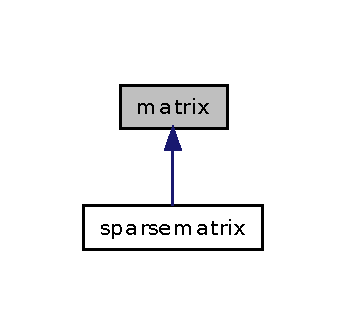
\includegraphics[width=166pt]{a00037}
\end{center}
\end{figure}


\subsection{Detailed Description}
A matlab matrix. 

This class is an artificially created class in doxygen to allow more precise type declarations 

The documentation for this class was generated from the following file\-:\begin{DoxyCompactItemize}
\item 
\hyperlink{a00016}{class\-\_\-substitutes.\-c}\end{DoxyCompactItemize}

\hypertarget{a00011}{\section{rowvec Class Reference}
\label{a00011}\index{rowvec@{rowvec}}
}


A matlab row vector.  




\subsection{Detailed Description}
A matlab row vector. 

This class is an artificially created class in doxygen to allow more precise type declarations 

The documentation for this class was generated from the following file\-:\begin{DoxyCompactItemize}
\item 
\hyperlink{a00016}{class\-\_\-substitutes.\-c}\end{DoxyCompactItemize}

\input{a00012}
\input{a00013}
\hypertarget{a00014}{\section{varargin Class Reference}
\label{a00014}\index{varargin@{varargin}}
}


A variable number of input arguments.  




\subsection{Detailed Description}
A variable number of input arguments. 

This class is an artificially created class in doxygen to allow more precise type declarations.

For more information about the varargin argument see the \href{http://www.mathworks.de/help/techdoc/ref/varargin.html}{\tt Mat\-Lab documentation on varargin}. 

The documentation for this class was generated from the following file\-:\begin{DoxyCompactItemize}
\item 
\hyperlink{a00016}{class\-\_\-substitutes.\-c}\end{DoxyCompactItemize}

\hypertarget{a00015}{\section{varargout Class Reference}
\label{a00015}\index{varargout@{varargout}}
}


A variable number of output arguments.  




\subsection{Detailed Description}
A variable number of output arguments. 

This class is an artificially created class in doxygen to allow more precise type declarations.

For more information about the varargout argument see the \href{http://www.mathworks.de/help/techdoc/ref/varargout.html}{\tt Mat\-Lab documentation on varargout}. 

The documentation for this class was generated from the following file\-:\begin{DoxyCompactItemize}
\item 
\hyperlink{a00016}{class\-\_\-substitutes.\-c}\end{DoxyCompactItemize}

\chapter{File Documentation}
\hypertarget{a00016}{\section{class\-\_\-substitutes.\-c File Reference}
\label{a00016}\index{class\-\_\-substitutes.\-c@{class\-\_\-substitutes.\-c}}
}
\subsection*{Classes}
\begin{DoxyCompactItemize}
\item 
class \hyperlink{a00010}{matrix}
\begin{DoxyCompactList}\small\item\em A matlab matrix. \end{DoxyCompactList}\item 
class \hyperlink{a00012}{sparsematrix}
\begin{DoxyCompactList}\small\item\em A matlab sparse matrix. \end{DoxyCompactList}\item 
class \hyperlink{a00007}{handle}
\begin{DoxyCompactList}\small\item\em Matlab's base handle class (documentation generation substitute) \end{DoxyCompactList}\end{DoxyCompactItemize}

\hypertarget{a00017}{\section{developers.\-c File Reference}
\label{a00017}\index{developers.\-c@{developers.\-c}}
}

\hypertarget{a00018}{\section{dirichlet\-\_\-int.\-m File Reference}
\label{a00018}\index{dirichlet\-\_\-int.\-m@{dirichlet\-\_\-int.\-m}}
}


Calcula la integral total de frontera para problemas no homogeneos \[ \int_{ \partial \Omega} \, n \times \curl{\bds{u}} \cdot \bds{\phi}_j \, \mathrm{d}x \] donde $ \bds{\phi}_i $ es una función base (elementos de Whitney en 2\-D)  


\subsection*{Functions}
\begin{DoxyCompactItemize}
\item 
mlhs\-Inner\-Subst\\*
$<$ matlabtypesubstitute, F\-T $>$ \hyperlink{a00018_a9621b6ebc3bb5bf12c40441f3ac49296}{dirichlet\-\_\-int} (matlabtypesubstitute u, matlabtypesubstitute rhs, matlabtypesubstitute Z)
\begin{DoxyCompactList}\small\item\em Calcula la integral total de frontera para problemas no homogeneos \[ \int_{ \partial \Omega} \, n \times \curl{\bds{u}} \cdot \bds{\phi}_j \, \mathrm{d}x \] donde $ \bds{\phi}_i $ es una función base (elementos de Whitney en 2\-D) \end{DoxyCompactList}\item 
mlhs\-Inner\-Subst\\*
$<$ matlabtypesubstitute, F $>$ \hyperlink{a00018_a7cf2e1a404469b4ff7462d92a66e67b0}{mtoc\-\_\-subst\-\_\-dirichlet\-\_\-int\-\_\-m\-\_\-tsbus\-\_\-cotm\-\_\-int\-\_\-lado} (matlabtypesubstitute u, matlabtypesubstitute k, matlabtypesubstitute j, matlabtypesubstitute rhs, matlabtypesubstitute Z)
\begin{DoxyCompactList}\small\item\em Calcula la integral de frontera para problemas no homogeneos \[ \int_{\Gamma_k}\, n \times f(x) \bds{\phi}_j \, \mathrm{d}x \] sobre el elemento $ T_k $ donde $ \bds{\phi}_i $ es una función base (elementos de Whitney en 2\-D) \end{DoxyCompactList}\item 
mlhs\-Inner\-Subst\\*
$<$ matlabtypesubstitute, Es $>$ \hyperlink{a00018_a90097a853874acfe2f32c2a6816c75ff}{mtoc\-\_\-subst\-\_\-dirichlet\-\_\-int\-\_\-m\-\_\-tsbus\-\_\-cotm\-\_\-ncurl\-\_\-u} (matlabtypesubstitute xs, matlabtypesubstitute n, matlabtypesubstitute rhs)
\end{DoxyCompactItemize}


\subsection{Detailed Description}
Calcula la integral total de frontera para problemas no homogeneos \[ \int_{ \partial \Omega} \, n \times \curl{\bds{u}} \cdot \bds{\phi}_j \, \mathrm{d}x \] donde $ \bds{\phi}_i $ es una función base (elementos de Whitney en 2\-D) 

\subsection{Function Documentation}
\hypertarget{a00018_a9621b6ebc3bb5bf12c40441f3ac49296}{\index{dirichlet\-\_\-int.\-m@{dirichlet\-\_\-int.\-m}!dirichlet\-\_\-int@{dirichlet\-\_\-int}}
\index{dirichlet\-\_\-int@{dirichlet\-\_\-int}!dirichlet_int.m@{dirichlet\-\_\-int.\-m}}
\subsubsection[{dirichlet\-\_\-int}]{\setlength{\rightskip}{0pt plus 5cm}mlhs\-Inner\-Subst$<$ matlabtypesubstitute, F\-T $>$ {\bf dirichlet\-\_\-int} (
\begin{DoxyParamCaption}
\item[{matlabtypesubstitute}]{u, }
\item[{matlabtypesubstitute}]{rhs, }
\item[{matlabtypesubstitute}]{Z}
\end{DoxyParamCaption}
)}}\label{a00018_a9621b6ebc3bb5bf12c40441f3ac49296}


Calcula la integral total de frontera para problemas no homogeneos \[ \int_{ \partial \Omega} \, n \times \curl{\bds{u}} \cdot \bds{\phi}_j \, \mathrm{d}x \] donde $ \bds{\phi}_i $ es una función base (elementos de Whitney en 2\-D) 

\begin{DoxyAuthor}{Author}
Ricardo Prato 

Catalina Dominguez 
\end{DoxyAuthor}
\begin{DoxyDate}{Date}
2012-\/04-\/25
\end{DoxyDate}

\begin{DoxyParams}{Parameters}
{\em u} & {\bfseries Estructura} \\
\hline
{\em rhs} & Id. del lado derecho \\
\hline
{\em Z} & Estructura para el tiempo\\
\hline
\end{DoxyParams}

\begin{DoxyRetVals}{Return values}
{\em F\-T} & F\-T \\
\hline
{\em F} & Matriz. Lado derecho\\
\hline
\end{DoxyRetVals}
\begin{DoxyParagraph}{Required fields of u\-:}

\end{DoxyParagraph}
\hypertarget{a00018_a7cf2e1a404469b4ff7462d92a66e67b0}{\index{dirichlet\-\_\-int.\-m@{dirichlet\-\_\-int.\-m}!mtoc\-\_\-subst\-\_\-dirichlet\-\_\-int\-\_\-m\-\_\-tsbus\-\_\-cotm\-\_\-int\-\_\-lado@{mtoc\-\_\-subst\-\_\-dirichlet\-\_\-int\-\_\-m\-\_\-tsbus\-\_\-cotm\-\_\-int\-\_\-lado}}
\index{mtoc\-\_\-subst\-\_\-dirichlet\-\_\-int\-\_\-m\-\_\-tsbus\-\_\-cotm\-\_\-int\-\_\-lado@{mtoc\-\_\-subst\-\_\-dirichlet\-\_\-int\-\_\-m\-\_\-tsbus\-\_\-cotm\-\_\-int\-\_\-lado}!dirichlet_int.m@{dirichlet\-\_\-int.\-m}}
\subsubsection[{mtoc\-\_\-subst\-\_\-dirichlet\-\_\-int\-\_\-m\-\_\-tsbus\-\_\-cotm\-\_\-int\-\_\-lado}]{\setlength{\rightskip}{0pt plus 5cm}mlhs\-Inner\-Subst$<$ matlabtypesubstitute, F $>$ {\bf mtoc\-\_\-subst\-\_\-dirichlet\-\_\-int\-\_\-m\-\_\-tsbus\-\_\-cotm\-\_\-int\-\_\-lado} (
\begin{DoxyParamCaption}
\item[{matlabtypesubstitute}]{u, }
\item[{matlabtypesubstitute}]{k, }
\item[{matlabtypesubstitute}]{j, }
\item[{matlabtypesubstitute}]{rhs, }
\item[{matlabtypesubstitute}]{Z}
\end{DoxyParamCaption}
)}}\label{a00018_a7cf2e1a404469b4ff7462d92a66e67b0}


Calcula la integral de frontera para problemas no homogeneos \[ \int_{\Gamma_k}\, n \times f(x) \bds{\phi}_j \, \mathrm{d}x \] sobre el elemento $ T_k $ donde $ \bds{\phi}_i $ es una función base (elementos de Whitney en 2\-D) 

\begin{DoxyAuthor}{Author}
Ricardo Prato 

Catalina Dominguez 
\end{DoxyAuthor}
\begin{DoxyDate}{Date}
2012-\/04-\/25
\end{DoxyDate}

\begin{DoxyParams}{Parameters}
{\em u} & {\bfseries Estructura} \\
\hline
{\em k} & Id del elemento de frontera \\
\hline
{\em j} & Id del elemento de frontera \\
\hline
{\em rhs} & Id. del lado derecho \\
\hline
{\em Z} & Estructura. Información del tiempo.\\
\hline
\end{DoxyParams}

\begin{DoxyRetVals}{Return values}
{\em F} & Matriz. Lado derecho\\
\hline
\end{DoxyRetVals}
\begin{DoxyParagraph}{Required fields of Z\-:}

\end{DoxyParagraph}
\begin{DoxyParagraph}{Required fields of u\-:}

\end{DoxyParagraph}
\hypertarget{a00018_a90097a853874acfe2f32c2a6816c75ff}{\index{dirichlet\-\_\-int.\-m@{dirichlet\-\_\-int.\-m}!mtoc\-\_\-subst\-\_\-dirichlet\-\_\-int\-\_\-m\-\_\-tsbus\-\_\-cotm\-\_\-ncurl\-\_\-u@{mtoc\-\_\-subst\-\_\-dirichlet\-\_\-int\-\_\-m\-\_\-tsbus\-\_\-cotm\-\_\-ncurl\-\_\-u}}
\index{mtoc\-\_\-subst\-\_\-dirichlet\-\_\-int\-\_\-m\-\_\-tsbus\-\_\-cotm\-\_\-ncurl\-\_\-u@{mtoc\-\_\-subst\-\_\-dirichlet\-\_\-int\-\_\-m\-\_\-tsbus\-\_\-cotm\-\_\-ncurl\-\_\-u}!dirichlet_int.m@{dirichlet\-\_\-int.\-m}}
\subsubsection[{mtoc\-\_\-subst\-\_\-dirichlet\-\_\-int\-\_\-m\-\_\-tsbus\-\_\-cotm\-\_\-ncurl\-\_\-u}]{\setlength{\rightskip}{0pt plus 5cm}mlhs\-Inner\-Subst$<$matlabtypesubstitute,Es$>$ {\bf mtoc\-\_\-subst\-\_\-dirichlet\-\_\-int\-\_\-m\-\_\-tsbus\-\_\-cotm\-\_\-ncurl\-\_\-u} (
\begin{DoxyParamCaption}
\item[{matlabtypesubstitute}]{xs, }
\item[{matlabtypesubstitute}]{n, }
\item[{matlabtypesubstitute}]{rhs}
\end{DoxyParamCaption}
)}}\label{a00018_a90097a853874acfe2f32c2a6816c75ff}

\hypertarget{a00019}{\section{E\-\_\-error3.\-m File Reference}
\label{a00019}\index{E\-\_\-error3.\-m@{E\-\_\-error3.\-m}}
}


Calcula el error (en caso de tener solución exacta) \[ \Vert E-E_h \Vert_{H(curl,\Omega)} \].  


\subsection*{Functions}
\begin{DoxyCompactItemize}
\item 
mlhs\-Inner\-Subst\\*
$<$ matlabtypesubstitute, err $>$ \hyperlink{a00019_a29de8f298869566020d8775a9b41b8c4}{E\-\_\-error3} (matlabtypesubstitute u, matlabtypesubstitute Z, matlabtypesubstitute xh, matlabtypesubstitute rhs)
\begin{DoxyCompactList}\small\item\em Calcula el error (en caso de tener solución exacta) \[ \Vert E-E_h \Vert_{H(curl,\Omega)} \]. \end{DoxyCompactList}\item 
mlhs\-Inner\-Subst\\*
$<$ matlabtypesubstitute, saa $>$ \hyperlink{a00019_a97545bbb7f20a11107225170ca296c3b}{mtoc\-\_\-subst\-\_\-\-E\-\_\-error3\-\_\-m\-\_\-tsbus\-\_\-cotm\-\_\-checkwhitney} (matlabtypesubstitute u, matlabtypesubstitute k, matlabtypesubstitute ld, matlabtypesubstitute id, matlabtypesubstitute rhs, matlabtypesubstitute tk)
\begin{DoxyCompactList}\small\item\em Determina el Id. del lado al que esta asociado la función de Whitney. \end{DoxyCompactList}\end{DoxyCompactItemize}


\subsection{Detailed Description}
Calcula el error (en caso de tener solución exacta) \[ \Vert E-E_h \Vert_{H(curl,\Omega)} \]. 

\subsection{Function Documentation}
\hypertarget{a00019_a29de8f298869566020d8775a9b41b8c4}{\index{E\-\_\-error3.\-m@{E\-\_\-error3.\-m}!E\-\_\-error3@{E\-\_\-error3}}
\index{E\-\_\-error3@{E\-\_\-error3}!E_error3.m@{E\-\_\-error3.\-m}}
\subsubsection[{E\-\_\-error3}]{\setlength{\rightskip}{0pt plus 5cm}mlhs\-Inner\-Subst$<$ matlabtypesubstitute, err $>$ {\bf E\-\_\-error3} (
\begin{DoxyParamCaption}
\item[{matlabtypesubstitute}]{u, }
\item[{matlabtypesubstitute}]{Z, }
\item[{matlabtypesubstitute}]{xh, }
\item[{matlabtypesubstitute}]{rhs}
\end{DoxyParamCaption}
)}}\label{a00019_a29de8f298869566020d8775a9b41b8c4}


Calcula el error (en caso de tener solución exacta) \[ \Vert E-E_h \Vert_{H(curl,\Omega)} \]. 

sobre el elemento $ T_k $ donde $ \bds{\phi}_i $ es una función base (elementos de Whitney en 2\-D)

\begin{DoxyAuthor}{Author}
Ricardo Prato 

Catalina Dominguez 
\end{DoxyAuthor}
\begin{DoxyDate}{Date}
2012-\/03-\/30
\end{DoxyDate}

\begin{DoxyParams}{Parameters}
{\em u} & {\bfseries Estructura} \\
\hline
{\em Z} & Estructura para el tiempo \\
\hline
{\em xh} & Solución aproximada \\
\hline
{\em rhs} & Id. de la solución exacta\\
\hline
\end{DoxyParams}

\begin{DoxyRetVals}{Return values}
{\em err} & Matriz. Error\\
\hline
\end{DoxyRetVals}
\begin{DoxyParagraph}{Required fields of Z\-:}

\end{DoxyParagraph}
\begin{DoxyParagraph}{Required fields of u\-:}

\end{DoxyParagraph}
\hypertarget{a00019_a97545bbb7f20a11107225170ca296c3b}{\index{E\-\_\-error3.\-m@{E\-\_\-error3.\-m}!mtoc\-\_\-subst\-\_\-\-E\-\_\-error3\-\_\-m\-\_\-tsbus\-\_\-cotm\-\_\-checkwhitney@{mtoc\-\_\-subst\-\_\-\-E\-\_\-error3\-\_\-m\-\_\-tsbus\-\_\-cotm\-\_\-checkwhitney}}
\index{mtoc\-\_\-subst\-\_\-\-E\-\_\-error3\-\_\-m\-\_\-tsbus\-\_\-cotm\-\_\-checkwhitney@{mtoc\-\_\-subst\-\_\-\-E\-\_\-error3\-\_\-m\-\_\-tsbus\-\_\-cotm\-\_\-checkwhitney}!E_error3.m@{E\-\_\-error3.\-m}}
\subsubsection[{mtoc\-\_\-subst\-\_\-\-E\-\_\-error3\-\_\-m\-\_\-tsbus\-\_\-cotm\-\_\-checkwhitney}]{\setlength{\rightskip}{0pt plus 5cm}mlhs\-Inner\-Subst$<$ matlabtypesubstitute, saa $>$ {\bf mtoc\-\_\-subst\-\_\-\-E\-\_\-error3\-\_\-m\-\_\-tsbus\-\_\-cotm\-\_\-checkwhitney} (
\begin{DoxyParamCaption}
\item[{matlabtypesubstitute}]{u, }
\item[{matlabtypesubstitute}]{k, }
\item[{matlabtypesubstitute}]{ld, }
\item[{matlabtypesubstitute}]{id, }
\item[{matlabtypesubstitute}]{rhs, }
\item[{matlabtypesubstitute}]{tk}
\end{DoxyParamCaption}
)}}\label{a00019_a97545bbb7f20a11107225170ca296c3b}


Determina el Id. del lado al que esta asociado la función de Whitney. 

\begin{DoxyAuthor}{Author}
Ricardo Prato 
\end{DoxyAuthor}
\begin{DoxyDate}{Date}
2012-\/04-\/25
\end{DoxyDate}

\begin{DoxyParams}{Parameters}
{\em u} & {\bfseries Estructura} \\
\hline
{\em k} & Id. del elemento \\
\hline
{\em ld} & Id. del lado \\
\hline
{\em id} & numero de co \\
\hline
{\em rhs} & Id. de la solución exacta \\
\hline
{\em tk} & Tiempo\\
\hline
\end{DoxyParams}

\begin{DoxyRetVals}{Return values}
{\em saa} & Relacion lado-\/función\\
\hline
\end{DoxyRetVals}
\begin{DoxyParagraph}{Required fields of u\-:}

\end{DoxyParagraph}

\input{a00020}
\input{a00021}
\hypertarget{a00022}{\section{funciones.\-m File Reference}
\label{a00022}\index{funciones.\-m@{funciones.\-m}}
}


String de la función exacta utilizada. Por ejemplo,.  


\subsection*{Functions}
\begin{DoxyCompactItemize}
\item 
mlhs\-Inner\-Subst\\*
$<$ matlabtypesubstitute, value $>$ \hyperlink{a00022_a0e5b67397a954c71651f4b0fb44bb8fa}{funciones} (matlabtypesubstitute rhs)
\begin{DoxyCompactList}\small\item\em String de la función exacta utilizada. Por ejemplo,. \end{DoxyCompactList}\end{DoxyCompactItemize}


\subsection{Detailed Description}
String de la función exacta utilizada. Por ejemplo,. 
\begin{DoxyCode}
 >> funciones(80)  
\end{DoxyCode}
 \begin{DoxyVerb}     E:=sin(t)*[x*y * (1 - x) * (1 - y)),0]\end{DoxyVerb}
 Parameters\-: rhs\-: Entero. Id. de la función exacta 

\subsection{Function Documentation}
\hypertarget{a00022_a0e5b67397a954c71651f4b0fb44bb8fa}{\index{funciones.\-m@{funciones.\-m}!funciones@{funciones}}
\index{funciones@{funciones}!funciones.m@{funciones.\-m}}
\subsubsection[{funciones}]{\setlength{\rightskip}{0pt plus 5cm}mlhs\-Inner\-Subst$<$ matlabtypesubstitute, value $>$ {\bf funciones} (
\begin{DoxyParamCaption}
\item[{matlabtypesubstitute}]{rhs}
\end{DoxyParamCaption}
)}}\label{a00022_a0e5b67397a954c71651f4b0fb44bb8fa}


String de la función exacta utilizada. Por ejemplo,. 


\begin{DoxyCode}
 >> funciones(80)  
\end{DoxyCode}
 \begin{DoxyVerb}     E:=sin(t)*[x*y * (1 - x) * (1 - y)),0]\end{DoxyVerb}
 Parameters\-: rhs\-: Entero. Id. de la función exacta

\begin{DoxyAuthor}{Author}
Catalina Dominguez 
\end{DoxyAuthor}
\begin{DoxyDate}{Date}
2012-\/03-\/25
\end{DoxyDate}

\begin{DoxyParams}{Parameters}
{\em rhs} & rhs\\
\hline
\end{DoxyParams}

\begin{DoxyRetVals}{Return values}
{\em value} & String . Forma de la solución exacta \\
\hline
\end{DoxyRetVals}

\hypertarget{a00023}{\section{gauss.\-m File Reference}
\label{a00023}\index{gauss.\-m@{gauss.\-m}}
}


Genera los puntos $ x_i $ y los pesos $ w_i $ para una cuadratura Gauss-\/\-Legendre \[ \int_{a}^b W(x) \cdot f(t) dt \approx \sum_{i=1}^{n} w_i \, f(x_i) \] siguiendo lo propuesto en la sección 4.\-6 de \par
 Numerical Recipes\-: The Art of Scientific Computing \par
 Third Edition (2007) \par
 Cambridge University Press \par
 I\-S\-B\-N-\/10\-: 0521880688.  


\subsection*{Functions}
\begin{DoxyCompactItemize}
\item 
mlhs\-Subst$<$ mlhs\-Inner\-Subst\\*
$<$ matlabtypesubstitute, x $>$\\*
,mlhs\-Inner\-Subst\\*
$<$ matlabtypesubstitute, w $>$ $>$ \hyperlink{a00023_a5cac7731040a0693793dfebeeb1bf85b}{gauss} (matlabtypesubstitute n)
\begin{DoxyCompactList}\small\item\em Genera los puntos $ x_i $ y los pesos $ w_i $ para una cuadratura Gauss-\/\-Legendre \[ \int_{a}^b W(x) \cdot f(t) dt \approx \sum_{i=1}^{n} w_i \, f(x_i) \] siguiendo lo propuesto en la sección 4.\-6 de \par
 Numerical Recipes\-: The Art of Scientific Computing \par
 Third Edition (2007) \par
 Cambridge University Press \par
 I\-S\-B\-N-\/10\-: 0521880688. \end{DoxyCompactList}\end{DoxyCompactItemize}


\subsection{Detailed Description}
Genera los puntos $ x_i $ y los pesos $ w_i $ para una cuadratura Gauss-\/\-Legendre \[ \int_{a}^b W(x) \cdot f(t) dt \approx \sum_{i=1}^{n} w_i \, f(x_i) \] siguiendo lo propuesto en la sección 4.\-6 de \par
 Numerical Recipes\-: The Art of Scientific Computing \par
 Third Edition (2007) \par
 Cambridge University Press \par
 I\-S\-B\-N-\/10\-: 0521880688. 

\subsection{Function Documentation}
\hypertarget{a00023_a5cac7731040a0693793dfebeeb1bf85b}{\index{gauss.\-m@{gauss.\-m}!gauss@{gauss}}
\index{gauss@{gauss}!gauss.m@{gauss.\-m}}
\subsubsection[{gauss}]{\setlength{\rightskip}{0pt plus 5cm}mlhs\-Subst$<$ mlhs\-Inner\-Subst$<$ matlabtypesubstitute, x $>$,mlhs\-Inner\-Subst$<$ matlabtypesubstitute, w $>$ $>$ {\bf gauss} (
\begin{DoxyParamCaption}
\item[{matlabtypesubstitute}]{n}
\end{DoxyParamCaption}
)}}\label{a00023_a5cac7731040a0693793dfebeeb1bf85b}


Genera los puntos $ x_i $ y los pesos $ w_i $ para una cuadratura Gauss-\/\-Legendre \[ \int_{a}^b W(x) \cdot f(t) dt \approx \sum_{i=1}^{n} w_i \, f(x_i) \] siguiendo lo propuesto en la sección 4.\-6 de \par
 Numerical Recipes\-: The Art of Scientific Computing \par
 Third Edition (2007) \par
 Cambridge University Press \par
 I\-S\-B\-N-\/10\-: 0521880688. 


\begin{DoxyParams}{Parameters}
{\em n} & número de puntos de cuadratura\\
\hline
\end{DoxyParams}

\begin{DoxyRetVals}{Return values}
{\em x} & Puntos de cuadratura \\
\hline
{\em w} & Pesos Gaussianos \\
\hline
\end{DoxyRetVals}
\begin{DoxyAuthor}{Author}
Ricardo Prato 

Catalina Dominguez 
\end{DoxyAuthor}
\begin{DoxyDate}{Date}
2012-\/03-\/24 
\end{DoxyDate}

\hypertarget{a00024}{\section{int\-\_\-time.\-m File Reference}
\label{a00024}\index{int\-\_\-time.\-m@{int\-\_\-time.\-m}}
}


Calcula el valor de las integrales \begin{eqnarray*} I_1 =\int_{t_{n-1}}^{t_{n}} (t-t_{m})\cdot t_{n} \cdot g(t) \, dt &\qquad& I_2 =\int_{t_{n-1}}^{t_{n}} (t-t_{m})\cdot t_{n} \cdot g^{\prime}(t) \, dt \\[3mm] I_3 = \int_{t_{n-1}}^{t_{n}} (t-t_{n-1})\cdot t_{n} \cdot g(t) \, dt &\qquad& I_4 = \int_{t_{n-1}}^{t_{n}} (t-t_{n-1})\cdot t_{n} \cdot g^{\prime}(t) \, dt \\[3mm] I_5 = \int_{t_{n-1}}^{t_{n}} (t-t_{n-1})\cdot t_{m} \cdot g(t) \, dt &\qquad& I_6 = \int_{t_{n-1}}^{t_{n}} (t-t_{n-1})\cdot t_{m} \cdot g^{\prime}(t) \, dt \ \end{eqnarray*}.  


\subsection*{Functions}
\begin{DoxyCompactItemize}
\item 
mlhs\-Inner\-Subst\\*
$<$ matlabtypesubstitute, Z $>$ \hyperlink{a00024_ac36b34d8a822fd1d7a80a5bc546a0ca2}{int\-\_\-time} (matlabtypesubstitute Z)
\begin{DoxyCompactList}\small\item\em Calcula el valor de las integrales \begin{eqnarray*} I_1 =\int_{t_{n-1}}^{t_{n}} (t-t_{m})\cdot t_{n} \cdot g(t) \, dt &\qquad& I_2 =\int_{t_{n-1}}^{t_{n}} (t-t_{m})\cdot t_{n} \cdot g^{\prime}(t) \, dt \\[3mm] I_3 = \int_{t_{n-1}}^{t_{n}} (t-t_{n-1})\cdot t_{n} \cdot g(t) \, dt &\qquad& I_4 = \int_{t_{n-1}}^{t_{n}} (t-t_{n-1})\cdot t_{n} \cdot g^{\prime}(t) \, dt \\[3mm] I_5 = \int_{t_{n-1}}^{t_{n}} (t-t_{n-1})\cdot t_{m} \cdot g(t) \, dt &\qquad& I_6 = \int_{t_{n-1}}^{t_{n}} (t-t_{n-1})\cdot t_{m} \cdot g^{\prime}(t) \, dt \ \end{eqnarray*}. \end{DoxyCompactList}\end{DoxyCompactItemize}


\subsection{Detailed Description}
Calcula el valor de las integrales \begin{eqnarray*} I_1 =\int_{t_{n-1}}^{t_{n}} (t-t_{m})\cdot t_{n} \cdot g(t) \, dt &\qquad& I_2 =\int_{t_{n-1}}^{t_{n}} (t-t_{m})\cdot t_{n} \cdot g^{\prime}(t) \, dt \\[3mm] I_3 = \int_{t_{n-1}}^{t_{n}} (t-t_{n-1})\cdot t_{n} \cdot g(t) \, dt &\qquad& I_4 = \int_{t_{n-1}}^{t_{n}} (t-t_{n-1})\cdot t_{n} \cdot g^{\prime}(t) \, dt \\[3mm] I_5 = \int_{t_{n-1}}^{t_{n}} (t-t_{n-1})\cdot t_{m} \cdot g(t) \, dt &\qquad& I_6 = \int_{t_{n-1}}^{t_{n}} (t-t_{n-1})\cdot t_{m} \cdot g^{\prime}(t) \, dt \ \end{eqnarray*}. 

\subsection{Function Documentation}
\hypertarget{a00024_ac36b34d8a822fd1d7a80a5bc546a0ca2}{\index{int\-\_\-time.\-m@{int\-\_\-time.\-m}!int\-\_\-time@{int\-\_\-time}}
\index{int\-\_\-time@{int\-\_\-time}!int_time.m@{int\-\_\-time.\-m}}
\subsubsection[{int\-\_\-time}]{\setlength{\rightskip}{0pt plus 5cm}mlhs\-Inner\-Subst$<$ matlabtypesubstitute, Z $>$ {\bf int\-\_\-time} (
\begin{DoxyParamCaption}
\item[{matlabtypesubstitute}]{Z}
\end{DoxyParamCaption}
)}}\label{a00024_ac36b34d8a822fd1d7a80a5bc546a0ca2}


Calcula el valor de las integrales \begin{eqnarray*} I_1 =\int_{t_{n-1}}^{t_{n}} (t-t_{m})\cdot t_{n} \cdot g(t) \, dt &\qquad& I_2 =\int_{t_{n-1}}^{t_{n}} (t-t_{m})\cdot t_{n} \cdot g^{\prime}(t) \, dt \\[3mm] I_3 = \int_{t_{n-1}}^{t_{n}} (t-t_{n-1})\cdot t_{n} \cdot g(t) \, dt &\qquad& I_4 = \int_{t_{n-1}}^{t_{n}} (t-t_{n-1})\cdot t_{n} \cdot g^{\prime}(t) \, dt \\[3mm] I_5 = \int_{t_{n-1}}^{t_{n}} (t-t_{n-1})\cdot t_{m} \cdot g(t) \, dt &\qquad& I_6 = \int_{t_{n-1}}^{t_{n}} (t-t_{n-1})\cdot t_{m} \cdot g^{\prime}(t) \, dt \ \end{eqnarray*}. 

\begin{DoxyAuthor}{Author}
Ricardo Prato 
\end{DoxyAuthor}
\begin{DoxyDate}{Date}
2012-\/04-\/01
\end{DoxyDate}

\begin{DoxyParams}{Parameters}
{\em Z} & {\bfseries Estructura} que contiene los datos del tiempo\\
\hline
\end{DoxyParams}

\begin{DoxyRetVals}{Return values}
{\em Z} & $[I_1,I_2,I_3,I_4,I_5,I_6]$\\
\hline
\end{DoxyRetVals}
\begin{DoxyParagraph}{Required fields of Z\-:}

\end{DoxyParagraph}
\begin{DoxyParagraph}{Generated fields of Z\-:}

\end{DoxyParagraph}

\hypertarget{a00025}{\section{malla01.\-m File Reference}
\label{a00025}\index{malla01.\-m@{malla01.\-m}}
}


Inicializa la geometria $ [0,1] \times [0,1] $ \par
.  


\subsection*{Functions}
\begin{DoxyCompactItemize}
\item 
mlhs\-Inner\-Subst\\*
$<$ matlabtypesubstitute, u $>$ \hyperlink{a00025_ac07ed38a984c8ec43246d07fd453cd8a}{malla01} (matlabtypesubstitute mode)
\begin{DoxyCompactList}\small\item\em Inicializa la geometria $ [0,1] \times [0,1] $ \par
. \end{DoxyCompactList}\end{DoxyCompactItemize}


\subsection{Detailed Description}
Inicializa la geometria $ [0,1] \times [0,1] $ \par
. 

\subsection{Function Documentation}
\hypertarget{a00025_ac07ed38a984c8ec43246d07fd453cd8a}{\index{malla01.\-m@{malla01.\-m}!malla01@{malla01}}
\index{malla01@{malla01}!malla01.m@{malla01.\-m}}
\subsubsection[{malla01}]{\setlength{\rightskip}{0pt plus 5cm}mlhs\-Inner\-Subst$<$ matlabtypesubstitute, u $>$ {\bf malla01} (
\begin{DoxyParamCaption}
\item[{matlabtypesubstitute}]{mode}
\end{DoxyParamCaption}
)}}\label{a00025_ac07ed38a984c8ec43246d07fd453cd8a}


Inicializa la geometria $ [0,1] \times [0,1] $ \par
. 




\begin{DoxyParams}{Parameters}
{\em mode} & Entero. Determina las condiciones de frontera
\begin{DoxyItemize}
\item mode=1\-: Dirichlet
\item mode $>$ 1\-: Condiciones Mixtas o Neumann
\end{DoxyItemize}\\
\hline
\end{DoxyParams}

\begin{DoxyRetVals}{Return values}
{\em u} & Estructura que contiene la malla y condiciones de frontera.\\
\hline
\end{DoxyRetVals}
\begin{DoxyParagraph}{Generated fields of u\-:}
\begin{DoxyItemize}
\item {\ttfamily u.\-node~---~} Matriz de orden (No. Puntos) x 2. Contiene las coordenadas de los puntos. \item {\ttfamily u.\-pnod~---~} Matriz de orden (No. Elementos) x 3. Contiene los nodos de cada elemento \item {\ttfamily u.\-numnod~---~} Entero. Número de nodos. \item {\ttfamily u.\-Dirich~---~} Matriz de orden (No. lados Dirichlet) x 2. Contiene los nodos de cada elemento de frontera con condición de Dirichlet. \item {\ttfamily u.\-Neumann~---~} Matriz de orden (No. lados Neumann) x 2. Contiene los nodos de cada elemento de frontera con condición de Neumann. \end{DoxyItemize}

\end{DoxyParagraph}
\begin{DoxyAuthor}{Author}
Ricardo Prato 

Catalina Dominguez 
\end{DoxyAuthor}
\begin{DoxyDate}{Date}
2012-\/03-\/20 
\end{DoxyDate}

\input{a00026}
\hypertarget{a00027}{\section{maxwell\-\_\-dgm2.\-m File Reference}
\label{a00027}\index{maxwell\-\_\-dgm2.\-m@{maxwell\-\_\-dgm2.\-m}}
}


Programa Principal para la aproximación de soluciones de un problema de Eddy current dependiente del tiempo \begin{eqnarray*} \frac{ \partial \bds{E}}{dt} + \curl{\Big ( \alpha \cdot \curl{E}\Big )} &=& f \mbox{ en $\Omega \times (0,T]$}\\ \bds{E} \times \bds{n} &=& g \mbox{ en $\partial \Omega \times (0,T]$}\\ \bds{E} &=& 0 \mbox{ en $ \Omega \times \{0\}$} \end{eqnarray*} en 2\-D utilizando para la discretización en el tiempo polinomios cuadráticos vía D\-G\-M y para la discrezación del espacio elementos de Whitney.  


\subsection*{Functions}
\begin{DoxyCompactItemize}
\item 
mlhs\-Inner\-Subst\\*
$<$ matlabtypesubstitute, u $>$ \hyperlink{a00027_aa1c23ee143ed2521278ea8594b5b3e8a}{maxwell\-\_\-dgm2} (matlabtypesubstitute mode, matlabtypesubstitute rhs, matlabtypesubstitute iter)
\begin{DoxyCompactList}\small\item\em Programa Principal para la aproximación de soluciones de un problema de Eddy current dependiente del tiempo \begin{eqnarray*} \frac{ \partial \bds{E}}{dt} + \curl{\Big ( \alpha \cdot \curl{E}\Big )} &=& f \mbox{ en $\Omega \times (0,T]$}\\ \bds{E} \times \bds{n} &=& g \mbox{ en $\partial \Omega \times (0,T]$}\\ \bds{E} &=& 0 \mbox{ en $ \Omega \times \{0\}$} \end{eqnarray*} en 2\-D utilizando para la discretización en el tiempo polinomios cuadráticos vía D\-G\-M y para la discrezación del espacio elementos de Whitney. \end{DoxyCompactList}\end{DoxyCompactItemize}


\subsection{Detailed Description}
Programa Principal para la aproximación de soluciones de un problema de Eddy current dependiente del tiempo \begin{eqnarray*} \frac{ \partial \bds{E}}{dt} + \curl{\Big ( \alpha \cdot \curl{E}\Big )} &=& f \mbox{ en $\Omega \times (0,T]$}\\ \bds{E} \times \bds{n} &=& g \mbox{ en $\partial \Omega \times (0,T]$}\\ \bds{E} &=& 0 \mbox{ en $ \Omega \times \{0\}$} \end{eqnarray*} en 2\-D utilizando para la discretización en el tiempo polinomios cuadráticos vía D\-G\-M y para la discrezación del espacio elementos de Whitney. 

\subsection{Function Documentation}
\hypertarget{a00027_aa1c23ee143ed2521278ea8594b5b3e8a}{\index{maxwell\-\_\-dgm2.\-m@{maxwell\-\_\-dgm2.\-m}!maxwell\-\_\-dgm2@{maxwell\-\_\-dgm2}}
\index{maxwell\-\_\-dgm2@{maxwell\-\_\-dgm2}!maxwell_dgm2.m@{maxwell\-\_\-dgm2.\-m}}
\subsubsection[{maxwell\-\_\-dgm2}]{\setlength{\rightskip}{0pt plus 5cm}mlhs\-Inner\-Subst$<$ matlabtypesubstitute, u $>$ {\bf maxwell\-\_\-dgm2} (
\begin{DoxyParamCaption}
\item[{matlabtypesubstitute}]{mode, }
\item[{matlabtypesubstitute}]{rhs, }
\item[{matlabtypesubstitute}]{iter}
\end{DoxyParamCaption}
)}}\label{a00027_aa1c23ee143ed2521278ea8594b5b3e8a}


Programa Principal para la aproximación de soluciones de un problema de Eddy current dependiente del tiempo \begin{eqnarray*} \frac{ \partial \bds{E}}{dt} + \curl{\Big ( \alpha \cdot \curl{E}\Big )} &=& f \mbox{ en $\Omega \times (0,T]$}\\ \bds{E} \times \bds{n} &=& g \mbox{ en $\partial \Omega \times (0,T]$}\\ \bds{E} &=& 0 \mbox{ en $ \Omega \times \{0\}$} \end{eqnarray*} en 2\-D utilizando para la discretización en el tiempo polinomios cuadráticos vía D\-G\-M y para la discrezación del espacio elementos de Whitney. 

\begin{DoxyAuthor}{Author}
Ricardo Prato 

Catalina Dominguez 
\end{DoxyAuthor}
\begin{DoxyDate}{Date}
2012-\/03-\/20
\end{DoxyDate}

\begin{DoxyParams}{Parameters}
{\em mode} & Determina las condiciones de frontera que se definen en el archivo malla$\ast$.m \par
 mode = 1 =$>$ Dirichlet \par
 mode $>$ 2 =$>$ Neumann o condiciones mixtas \\
\hline
{\em rhs} & Id de la función $f$ del lado derecho.\-Se define en el archivo \hyperlink{a00030}{rhs\-\_\-\-Maxw.\-m} \\
\hline
{\em iter} & Número de iteraciones\\
\hline
\end{DoxyParams}

\begin{DoxyRetVals}{Return values}
{\em u} & Estructura que contiene la información de mallas y solución para cada iteración \\
\hline
\end{DoxyRetVals}

\hypertarget{a00028}{\section{pt\-\_\-\-J.\-m File Reference}
\label{a00028}\index{pt\-\_\-\-J.\-m@{pt\-\_\-\-J.\-m}}
}


Define la función independiente del tiempo asociada al lado derecho \[ f(t,\bds{x})=-\partial_t \bds{J}=\sigma \partial_t \bds{E} + \frac{1}{\mu} \curl{\curl{E}} \] al definir $\bds{E} (t,\bds{x})=g(t) \cdot h(\bds{x})$.  


\subsection*{Functions}
\begin{DoxyCompactItemize}
\item 
mlhs\-Subst$<$ mlhs\-Inner\-Subst\\*
$<$ matlabtypesubstitute, pt\-J1 $>$\\*
,mlhs\-Inner\-Subst\\*
$<$ matlabtypesubstitute, pt\-J2 $>$ $>$ \hyperlink{a00028_ab3dcf8377a5fc5a2e5ce23db841507b7}{pt\-\_\-\-J} (matlabtypesubstitute u, matlabtypesubstitute rhs, matlabtypesubstitute xs)
\begin{DoxyCompactList}\small\item\em Define la función independiente del tiempo asociada al lado derecho \[ f(t,\bds{x})=-\partial_t \bds{J}=\sigma \partial_t \bds{E} + \frac{1}{\mu} \curl{\curl{E}} \] al definir $\bds{E} (t,\bds{x})=g(t) \cdot h(\bds{x})$. \end{DoxyCompactList}\end{DoxyCompactItemize}


\subsection{Detailed Description}
Define la función independiente del tiempo asociada al lado derecho \[ f(t,\bds{x})=-\partial_t \bds{J}=\sigma \partial_t \bds{E} + \frac{1}{\mu} \curl{\curl{E}} \] al definir $\bds{E} (t,\bds{x})=g(t) \cdot h(\bds{x})$. 

\subsection{Function Documentation}
\hypertarget{a00028_ab3dcf8377a5fc5a2e5ce23db841507b7}{\index{pt\-\_\-\-J.\-m@{pt\-\_\-\-J.\-m}!pt\-\_\-\-J@{pt\-\_\-\-J}}
\index{pt\-\_\-\-J@{pt\-\_\-\-J}!pt_J.m@{pt\-\_\-\-J.\-m}}
\subsubsection[{pt\-\_\-\-J}]{\setlength{\rightskip}{0pt plus 5cm}mlhs\-Subst$<$ mlhs\-Inner\-Subst$<$ matlabtypesubstitute, pt\-J1 $>$,mlhs\-Inner\-Subst$<$ matlabtypesubstitute, pt\-J2 $>$ $>$ {\bf pt\-\_\-\-J} (
\begin{DoxyParamCaption}
\item[{matlabtypesubstitute}]{u, }
\item[{matlabtypesubstitute}]{rhs, }
\item[{matlabtypesubstitute}]{xs}
\end{DoxyParamCaption}
)}}\label{a00028_ab3dcf8377a5fc5a2e5ce23db841507b7}


Define la función independiente del tiempo asociada al lado derecho \[ f(t,\bds{x})=-\partial_t \bds{J}=\sigma \partial_t \bds{E} + \frac{1}{\mu} \curl{\curl{E}} \] al definir $\bds{E} (t,\bds{x})=g(t) \cdot h(\bds{x})$. 


\begin{DoxyParams}{Parameters}
{\em u} & {\bfseries Estructura} \\
\hline
{\em rhs} & Id del lado derecho \\
\hline
{\em xs} & Punto\\
\hline
\end{DoxyParams}

\begin{DoxyRetVals}{Return values}
{\em pt\-J1} & $ \frac{1}{\mu} \curl{\curl{h(\bds{x})}} $ \\
\hline
{\em pt\-J2} & $ \sigma \partial_t {h(\bds{x})} $\\
\hline
\end{DoxyRetVals}
\begin{DoxyParagraph}{Required fields of u\-:}
\begin{DoxyItemize}
\item {\ttfamily u~---~} u.\-mumone u.\-sigma \end{DoxyItemize}

\end{DoxyParagraph}
\begin{DoxyAuthor}{Author}
Ricardo Prato 

Catalina Dominguez 
\end{DoxyAuthor}
\begin{DoxyDate}{Date}
2012-\/03-\/25 
\end{DoxyDate}

\hypertarget{a00029}{\section{refine\-R\-G\-B.\-m File Reference}
\label{a00029}\index{refine\-R\-G\-B.\-m@{refine\-R\-G\-B.\-m}}
}


Refina la malla provista por malla$\ast$.m utilizando un esquema red-\/green.  


\subsection*{Functions}
\begin{DoxyCompactItemize}
\item 
mlhs\-Subst$<$ mlhs\-Inner\-Subst\\*
$<$ matlabtypesubstitute, \\*
coordenadas $>$,mlhs\-Inner\-Subst\\*
$<$ matlabtypesubstitute, \\*
new\-Elements $>$,mlhs\-Inner\-Subst\\*
$<$ matlabtypesubstitute, \\*
\hyperlink{a00015}{varargout} $>$ $>$ \hyperlink{a00029_af36e1519bec7348bc4c928967c93800d}{refine\-R\-G\-B} (matlabtypesubstitute coordenadas, matlabtypesubstitute elements, matlabtypesubstitute \hyperlink{a00014}{varargin})
\begin{DoxyCompactList}\small\item\em Refina la malla provista por malla$\ast$.m utilizando un esquema red-\/green. \end{DoxyCompactList}\item 
mlhs\-Subst$<$ mlhs\-Inner\-Subst\\*
$<$ matlabtypesubstitute, \\*
edge2nodes $>$,mlhs\-Inner\-Subst\\*
$<$ matlabtypesubstitute, \\*
element2edges $>$,mlhs\-Inner\-Subst\\*
$<$ matlabtypesubstitute, \\*
\hyperlink{a00015}{varargout} $>$ $>$ \hyperlink{a00029_ab13f3537346ad3e10bb5f966d70ab360}{mtoc\-\_\-subst\-\_\-refine\-R\-G\-B\-\_\-m\-\_\-tsbus\-\_\-cotm\-\_\-\-Geometria} (matlabtypesubstitute elements, matlabtypesubstitute \hyperlink{a00014}{varargin})
\end{DoxyCompactItemize}


\subsection{Detailed Description}
Refina la malla provista por malla$\ast$.m utilizando un esquema red-\/green. 

\subsection{Function Documentation}
\hypertarget{a00029_ab13f3537346ad3e10bb5f966d70ab360}{\index{refine\-R\-G\-B.\-m@{refine\-R\-G\-B.\-m}!mtoc\-\_\-subst\-\_\-refine\-R\-G\-B\-\_\-m\-\_\-tsbus\-\_\-cotm\-\_\-\-Geometria@{mtoc\-\_\-subst\-\_\-refine\-R\-G\-B\-\_\-m\-\_\-tsbus\-\_\-cotm\-\_\-\-Geometria}}
\index{mtoc\-\_\-subst\-\_\-refine\-R\-G\-B\-\_\-m\-\_\-tsbus\-\_\-cotm\-\_\-\-Geometria@{mtoc\-\_\-subst\-\_\-refine\-R\-G\-B\-\_\-m\-\_\-tsbus\-\_\-cotm\-\_\-\-Geometria}!refineRGB.m@{refine\-R\-G\-B.\-m}}
\subsubsection[{mtoc\-\_\-subst\-\_\-refine\-R\-G\-B\-\_\-m\-\_\-tsbus\-\_\-cotm\-\_\-\-Geometria}]{\setlength{\rightskip}{0pt plus 5cm}mlhs\-Subst$<$mlhs\-Inner\-Subst$<$matlabtypesubstitute,edge2nodes$>$ ,mlhs\-Inner\-Subst$<$matlabtypesubstitute,element2edges$>$ ,mlhs\-Inner\-Subst$<$matlabtypesubstitute,{\bf varargout}$>$ $>$ {\bf mtoc\-\_\-subst\-\_\-refine\-R\-G\-B\-\_\-m\-\_\-tsbus\-\_\-cotm\-\_\-\-Geometria} (
\begin{DoxyParamCaption}
\item[{matlabtypesubstitute}]{elements, }
\item[{matlabtypesubstitute}]{varargin}
\end{DoxyParamCaption}
)}}\label{a00029_ab13f3537346ad3e10bb5f966d70ab360}
\hypertarget{a00029_af36e1519bec7348bc4c928967c93800d}{\index{refine\-R\-G\-B.\-m@{refine\-R\-G\-B.\-m}!refine\-R\-G\-B@{refine\-R\-G\-B}}
\index{refine\-R\-G\-B@{refine\-R\-G\-B}!refineRGB.m@{refine\-R\-G\-B.\-m}}
\subsubsection[{refine\-R\-G\-B}]{\setlength{\rightskip}{0pt plus 5cm}mlhs\-Subst$<$ mlhs\-Inner\-Subst$<$ matlabtypesubstitute, coordenadas $>$,mlhs\-Inner\-Subst$<$ matlabtypesubstitute, new\-Elements $>$,mlhs\-Inner\-Subst$<$ matlabtypesubstitute, {\bf varargout} $>$ $>$ {\bf refine\-R\-G\-B} (
\begin{DoxyParamCaption}
\item[{matlabtypesubstitute}]{coordenadas, }
\item[{matlabtypesubstitute}]{elements, }
\item[{matlabtypesubstitute}]{varargin}
\end{DoxyParamCaption}
)}}\label{a00029_af36e1519bec7348bc4c928967c93800d}


Refina la malla provista por malla$\ast$.m utilizando un esquema red-\/green. 



\begin{DoxyAuthor}{Author}
Ricardo Prato 

Catalina Dominguez 
\end{DoxyAuthor}
\begin{DoxyDate}{Date}
2011-\/08-\/17
\end{DoxyDate}

\begin{DoxyParams}{Parameters}
{\em coordenadas} & Matriz definida por u.\-node \\
\hline
{\em elements} & Matriz definida por u.\-pnod \\
\hline
{\em varargin} & posibilidades 
\begin{DoxyCode}
 ['Old u.Dirich', 'Old u.Neumann', 'Elementos marcados para refinar' ] 
\end{DoxyCode}
.\\
\hline
\end{DoxyParams}

\begin{DoxyRetVals}{Return values}
{\em coordenadas} & Matriz . Define un nuevo u.\-node \\
\hline
{\em new\-Elements} & Matriz . Define un nuevo u.\-pnod \\
\hline
{\em varargout} & posibilidades 
\begin{DoxyCode}
 ['new u.Dirich', 'new u.Neumann'] 
\end{DoxyCode}
. \\
\hline
\end{DoxyRetVals}

\hypertarget{a00030}{\section{rhs\-\_\-\-Maxw.\-m File Reference}
\label{a00030}\index{rhs\-\_\-\-Maxw.\-m@{rhs\-\_\-\-Maxw.\-m}}
}


Acopla la matriz de lado derecho local \[ \int_{\Omega}\,f(x) \bds{\phi}_j \, \mathrm{d}x \] donde $ \bds{\phi}_i $ es una función base (elementos de Whitney en 2\-D)  


\subsection*{Functions}
\begin{DoxyCompactItemize}
\item 
mlhs\-Inner\-Subst\\*
$<$ matlabtypesubstitute, F $>$ \hyperlink{a00030_a0611963c1c76c278859f84cefa8df08f}{rhs\-\_\-\-Maxw} (matlabtypesubstitute u, matlabtypesubstitute rhs, matlabtypesubstitute i, matlabtypesubstitute Z)
\begin{DoxyCompactList}\small\item\em Acopla la matriz de lado derecho local \[ \int_{\Omega}\,f(x) \bds{\phi}_j \, \mathrm{d}x \] donde $ \bds{\phi}_i $ es una función base (elementos de Whitney en 2\-D) \end{DoxyCompactList}\item 
mlhs\-Subst$<$ mlhs\-Inner\-Subst\\*
$<$ matlabtypesubstitute, B $>$\\*
,mlhs\-Inner\-Subst\\*
$<$ matlabtypesubstitute, C $>$ $>$ \hyperlink{a00030_a2848e8dd44d0e32a463abc0fd98e5d85}{mtoc\-\_\-subst\-\_\-rhs\-\_\-\-Maxw\-\_\-m\-\_\-tsbus\-\_\-cotm\-\_\-rhs\-\_\-\-Maxw\-\_\-elem} (matlabtypesubstitute u, matlabtypesubstitute rhs, matlabtypesubstitute k, matlabtypesubstitute a, matlabtypesubstitute b)
\begin{DoxyCompactList}\small\item\em Calcula la matriz de lado derecho local \[ \int_{T_i}\,f(x) \bds{\phi}_j \, \mathrm{d}x \] sobre el elemento $ T_k $ donde $ \bds{\phi}_i $ es una función base (elementos de Whitney en 2\-D) \end{DoxyCompactList}\end{DoxyCompactItemize}


\subsection{Detailed Description}
Acopla la matriz de lado derecho local \[ \int_{\Omega}\,f(x) \bds{\phi}_j \, \mathrm{d}x \] donde $ \bds{\phi}_i $ es una función base (elementos de Whitney en 2\-D) 

\subsection{Function Documentation}
\hypertarget{a00030_a2848e8dd44d0e32a463abc0fd98e5d85}{\index{rhs\-\_\-\-Maxw.\-m@{rhs\-\_\-\-Maxw.\-m}!mtoc\-\_\-subst\-\_\-rhs\-\_\-\-Maxw\-\_\-m\-\_\-tsbus\-\_\-cotm\-\_\-rhs\-\_\-\-Maxw\-\_\-elem@{mtoc\-\_\-subst\-\_\-rhs\-\_\-\-Maxw\-\_\-m\-\_\-tsbus\-\_\-cotm\-\_\-rhs\-\_\-\-Maxw\-\_\-elem}}
\index{mtoc\-\_\-subst\-\_\-rhs\-\_\-\-Maxw\-\_\-m\-\_\-tsbus\-\_\-cotm\-\_\-rhs\-\_\-\-Maxw\-\_\-elem@{mtoc\-\_\-subst\-\_\-rhs\-\_\-\-Maxw\-\_\-m\-\_\-tsbus\-\_\-cotm\-\_\-rhs\-\_\-\-Maxw\-\_\-elem}!rhs_Maxw.m@{rhs\-\_\-\-Maxw.\-m}}
\subsubsection[{mtoc\-\_\-subst\-\_\-rhs\-\_\-\-Maxw\-\_\-m\-\_\-tsbus\-\_\-cotm\-\_\-rhs\-\_\-\-Maxw\-\_\-elem}]{\setlength{\rightskip}{0pt plus 5cm}mlhs\-Subst$<$ mlhs\-Inner\-Subst$<$ matlabtypesubstitute, B $>$,mlhs\-Inner\-Subst$<$ matlabtypesubstitute, C $>$ $>$ {\bf mtoc\-\_\-subst\-\_\-rhs\-\_\-\-Maxw\-\_\-m\-\_\-tsbus\-\_\-cotm\-\_\-rhs\-\_\-\-Maxw\-\_\-elem} (
\begin{DoxyParamCaption}
\item[{matlabtypesubstitute}]{u, }
\item[{matlabtypesubstitute}]{rhs, }
\item[{matlabtypesubstitute}]{k, }
\item[{matlabtypesubstitute}]{a, }
\item[{matlabtypesubstitute}]{b}
\end{DoxyParamCaption}
)}}\label{a00030_a2848e8dd44d0e32a463abc0fd98e5d85}


Calcula la matriz de lado derecho local \[ \int_{T_i}\,f(x) \bds{\phi}_j \, \mathrm{d}x \] sobre el elemento $ T_k $ donde $ \bds{\phi}_i $ es una función base (elementos de Whitney en 2\-D) 


\begin{DoxyParams}{Parameters}
{\em u} & {\bfseries Estructura} \\
\hline
{\em rhs} & Id. de la solución exacta. \\
\hline
{\em k} & Id del elemento en la triangulación \\
\hline
{\em a} & Lado izquierdo del intervalo del tiempo \\
\hline
{\em b} & Lado derecho del intervalo del tiempo\\
\hline
\end{DoxyParams}

\begin{DoxyRetVals}{Return values}
{\em B} & Matriz. Lado derecho asociado al curl curl u \\
\hline
{\em C} & Matriz. Lado derecho asociado al $ \partial_t u $\\
\hline
\end{DoxyRetVals}
\begin{DoxyParagraph}{Required fields of u\-:}
\begin{DoxyItemize}
\item {\ttfamily u.\-pnod~---~} nodos globales asociadas al elemento i \item {\ttfamily u.\-node~---~} coordenadas de los elementos de la triangulación \end{DoxyItemize}

\end{DoxyParagraph}
\begin{DoxyAuthor}{Author}
Ricardo Prato 

Catalina Dominguez 
\end{DoxyAuthor}
\begin{DoxyDate}{Date}
2012-\/03-\/20 
\end{DoxyDate}
\hypertarget{a00030_a0611963c1c76c278859f84cefa8df08f}{\index{rhs\-\_\-\-Maxw.\-m@{rhs\-\_\-\-Maxw.\-m}!rhs\-\_\-\-Maxw@{rhs\-\_\-\-Maxw}}
\index{rhs\-\_\-\-Maxw@{rhs\-\_\-\-Maxw}!rhs_Maxw.m@{rhs\-\_\-\-Maxw.\-m}}
\subsubsection[{rhs\-\_\-\-Maxw}]{\setlength{\rightskip}{0pt plus 5cm}mlhs\-Inner\-Subst$<$ matlabtypesubstitute, F $>$ {\bf rhs\-\_\-\-Maxw} (
\begin{DoxyParamCaption}
\item[{matlabtypesubstitute}]{u, }
\item[{matlabtypesubstitute}]{rhs, }
\item[{matlabtypesubstitute}]{i, }
\item[{matlabtypesubstitute}]{Z}
\end{DoxyParamCaption}
)}}\label{a00030_a0611963c1c76c278859f84cefa8df08f}


Acopla la matriz de lado derecho local \[ \int_{\Omega}\,f(x) \bds{\phi}_j \, \mathrm{d}x \] donde $ \bds{\phi}_i $ es una función base (elementos de Whitney en 2\-D) 


\begin{DoxyParams}{Parameters}
{\em u} & {\bfseries Estructura} \\
\hline
{\em rhs} & Id. de la solución exacta. \\
\hline
{\em i} & Id del elemento en la triangulación \\
\hline
{\em Z} & Estructura del tiempo\\
\hline
\end{DoxyParams}

\begin{DoxyRetVals}{Return values}
{\em F} & Matriz. Lado derecho\\
\hline
\end{DoxyRetVals}
\begin{DoxyParagraph}{Required fields of u\-:}
\begin{DoxyItemize}
\item {\ttfamily u.\-pnod~---~} nodos globales asociadas al elemento i \item {\ttfamily u.\-node~---~} coordenadas de los elementos de la triangulación \end{DoxyItemize}

\end{DoxyParagraph}
\begin{DoxyAuthor}{Author}
Ricardo Prato 

Catalina Dominguez 
\end{DoxyAuthor}
\begin{DoxyDate}{Date}
2012-\/03-\/20
\end{DoxyDate}
\begin{DoxyParagraph}{Required fields of Z\-:}

\end{DoxyParagraph}

\hypertarget{a00031}{\section{shownu.\-m File Reference}
\label{a00031}\index{shownu.\-m@{shownu.\-m}}
}


Grafica la malla, y permite mostrar los elementos, nodos, y lados asociados a la misma.  


\subsection*{Functions}
\begin{DoxyCompactItemize}
\item 
noret\-::substitute \hyperlink{a00031_a5a6dfdfa880a93bff6a4798279a0a8e6}{shownu} (matlabtypesubstitute u, matlabtypesubstitute \hyperlink{a00014}{varargin})
\begin{DoxyCompactList}\small\item\em Grafica la malla, y permite mostrar los elementos, nodos, y lados asociados a la misma. \end{DoxyCompactList}\item 
mlhs\-Subst$<$ mlhs\-Inner\-Subst\\*
$<$ matlabtypesubstitute, \\*
numofnod $>$,mlhs\-Inner\-Subst\\*
$<$ matlabtypesubstitute, \\*
numofel $>$,mlhs\-Inner\-Subst\\*
$<$ matlabtypesubstitute, \\*
numofed $>$ $>$ \hyperlink{a00031_a7f9f7ccd03613cb0060385a015b085b5}{mtoc\-\_\-subst\-\_\-shownu\-\_\-m\-\_\-tsbus\-\_\-cotm\-\_\-check} (matlabtypesubstitute \hyperlink{a00014}{varargin})
\begin{DoxyCompactList}\small\item\em verifica la presencia los argumentos opcionales de la lista \end{DoxyCompactList}\end{DoxyCompactItemize}


\subsection{Detailed Description}
Grafica la malla, y permite mostrar los elementos, nodos, y lados asociados a la misma. 

\subsection{Function Documentation}
\hypertarget{a00031_a7f9f7ccd03613cb0060385a015b085b5}{\index{shownu.\-m@{shownu.\-m}!mtoc\-\_\-subst\-\_\-shownu\-\_\-m\-\_\-tsbus\-\_\-cotm\-\_\-check@{mtoc\-\_\-subst\-\_\-shownu\-\_\-m\-\_\-tsbus\-\_\-cotm\-\_\-check}}
\index{mtoc\-\_\-subst\-\_\-shownu\-\_\-m\-\_\-tsbus\-\_\-cotm\-\_\-check@{mtoc\-\_\-subst\-\_\-shownu\-\_\-m\-\_\-tsbus\-\_\-cotm\-\_\-check}!shownu.m@{shownu.\-m}}
\subsubsection[{mtoc\-\_\-subst\-\_\-shownu\-\_\-m\-\_\-tsbus\-\_\-cotm\-\_\-check}]{\setlength{\rightskip}{0pt plus 5cm}mlhs\-Subst$<$ mlhs\-Inner\-Subst$<$ matlabtypesubstitute, numofnod $>$,mlhs\-Inner\-Subst$<$ matlabtypesubstitute, numofel $>$,mlhs\-Inner\-Subst$<$ matlabtypesubstitute, numofed $>$ $>$ {\bf mtoc\-\_\-subst\-\_\-shownu\-\_\-m\-\_\-tsbus\-\_\-cotm\-\_\-check} (
\begin{DoxyParamCaption}
\item[{matlabtypesubstitute}]{varargin}
\end{DoxyParamCaption}
)}}\label{a00031_a7f9f7ccd03613cb0060385a015b085b5}


verifica la presencia los argumentos opcionales de la lista 


\begin{DoxyCode}
 ['nodos', 'elementos', 'lados' ] 
\end{DoxyCode}
.

\begin{DoxyAuthor}{Author}
Ricardo Prato 
\end{DoxyAuthor}
\begin{DoxyDate}{Date}
2012-\/03-\/20
\end{DoxyDate}

\begin{DoxyParams}{Parameters}
{\em varargin} & Alguno o todos los elementos de la lista 
\begin{DoxyCode}
 ['elementos', 'nodos', 'lados' ] 
\end{DoxyCode}
.\\
\hline
\end{DoxyParams}

\begin{DoxyRetVals}{Return values}
{\em numofnod} & Si nodos está es igual a 1, en otro caso 0 \\
\hline
{\em numofel} & Si elementos está es igual a 1, en otro caso 0 \\
\hline
{\em numofed} & Si lados está es igual a 1, en otro caso 0 \\
\hline
\end{DoxyRetVals}
\hypertarget{a00031_a5a6dfdfa880a93bff6a4798279a0a8e6}{\index{shownu.\-m@{shownu.\-m}!shownu@{shownu}}
\index{shownu@{shownu}!shownu.m@{shownu.\-m}}
\subsubsection[{shownu}]{\setlength{\rightskip}{0pt plus 5cm}noret\-::substitute {\bf shownu} (
\begin{DoxyParamCaption}
\item[{matlabtypesubstitute}]{u, }
\item[{matlabtypesubstitute}]{varargin}
\end{DoxyParamCaption}
)}}\label{a00031_a5a6dfdfa880a93bff6a4798279a0a8e6}


Grafica la malla, y permite mostrar los elementos, nodos, y lados asociados a la misma. 


\begin{DoxyParams}{Parameters}
{\em u} & {\bfseries Estructura} \\
\hline
{\em varargin} & String. Seleccione de la lista 
\begin{DoxyCode}
 ['elementos', 'nodos', 'lados' ] 
\end{DoxyCode}
.
\begin{DoxyItemize}
\item \begin{DoxyVerb}'elementos': ubica la numeración de los elementos \end{DoxyVerb}

\item \begin{DoxyVerb}'nodos' :ubica la numeración de los nodos  \end{DoxyVerb}

\item \begin{DoxyVerb}'lados' : ubica la numeración de los lados  \end{DoxyVerb}

\end{DoxyItemize}\\
\hline
\end{DoxyParams}
\begin{DoxyParagraph}{Required fields of u\-:}
\begin{DoxyItemize}
\item {\ttfamily u.\-node~---~} Matriz de orden (No. Puntos) x 2. Contiene las coordenadas de los puntos. \item {\ttfamily u.\-pnod~---~} Matriz de orden (No. Elementos) x 3. Contiene los nodos de cada elemento \item {\ttfamily u.\-numnod~---~} Entero. Número de nodos. \item {\ttfamily u.\-ed2nod~---~} Matriz de orden (No. lados) x 2. Contiene nodos globales asociados a cada lado. \end{DoxyItemize}

\end{DoxyParagraph}
\begin{DoxyAuthor}{Author}
Ricardo Prato 

Catalina Dominguez 
\end{DoxyAuthor}
\begin{DoxyDate}{Date}
2012-\/05-\/02 
\end{DoxyDate}

\hypertarget{a00032}{\section{Stiff\-\_\-\-Maxwell.\-m File Reference}
\label{a00032}\index{Stiff\-\_\-\-Maxwell.\-m@{Stiff\-\_\-\-Maxwell.\-m}}
}


Calcula la matriz de rigidez local $ ( \mrom{curl}\,\bds{\phi}_i,\mrom{curl}\,\bds{\phi}_j)_{T_k}$ sobre el elemento $ T_k $ donde $ \bds{\phi}_i $ es una función base (elementos de Whitney en 2\-D)  


\subsection*{Functions}
\begin{DoxyCompactItemize}
\item 
mlhs\-Subst$<$ mlhs\-Inner\-Subst\\*
$<$ matlabtypesubstitute, M $>$\\*
,mlhs\-Inner\-Subst\\*
$<$ matlabtypesubstitute, S $>$ $>$ \hyperlink{a00032_ae71a076bdebe889a60280f03734e4df0}{Stiff\-\_\-\-Maxwell} (matlabtypesubstitute u, matlabtypesubstitute k)
\begin{DoxyCompactList}\small\item\em Calcula la matriz de rigidez local $ ( \mrom{curl}\,\bds{\phi}_i,\mrom{curl}\,\bds{\phi}_j)_{T_k}$ sobre el elemento $ T_k $ donde $ \bds{\phi}_i $ es una función base (elementos de Whitney en 2\-D) \end{DoxyCompactList}\item 
mlhs\-Inner\-Subst\\*
$<$ matlabtypesubstitute, curl\-\_\-w $>$ \hyperlink{a00032_a8c5a4658d693facc7df0f7de9761b1ee}{mtoc\-\_\-subst\-\_\-\-Stiff\-\_\-\-Maxwell\-\_\-m\-\_\-tsbus\-\_\-cotm\-\_\-\-Curl\-\_\-whitney\-\_\-maxwell} (matlabtypesubstitute u, matlabtypesubstitute i, matlabtypesubstitute co)
\begin{DoxyCompactList}\small\item\em Calcula el rotacional $ \mrom{curl}\,\bds{\phi}_j$ sobre el elemento $ T_k $ donde $ \bds{\phi}_i $ es una función base (elementos de Whitney en 2\-D) \end{DoxyCompactList}\end{DoxyCompactItemize}


\subsection{Detailed Description}
Calcula la matriz de rigidez local $ ( \mrom{curl}\,\bds{\phi}_i,\mrom{curl}\,\bds{\phi}_j)_{T_k}$ sobre el elemento $ T_k $ donde $ \bds{\phi}_i $ es una función base (elementos de Whitney en 2\-D) 

\subsection{Function Documentation}
\hypertarget{a00032_a8c5a4658d693facc7df0f7de9761b1ee}{\index{Stiff\-\_\-\-Maxwell.\-m@{Stiff\-\_\-\-Maxwell.\-m}!mtoc\-\_\-subst\-\_\-\-Stiff\-\_\-\-Maxwell\-\_\-m\-\_\-tsbus\-\_\-cotm\-\_\-\-Curl\-\_\-whitney\-\_\-maxwell@{mtoc\-\_\-subst\-\_\-\-Stiff\-\_\-\-Maxwell\-\_\-m\-\_\-tsbus\-\_\-cotm\-\_\-\-Curl\-\_\-whitney\-\_\-maxwell}}
\index{mtoc\-\_\-subst\-\_\-\-Stiff\-\_\-\-Maxwell\-\_\-m\-\_\-tsbus\-\_\-cotm\-\_\-\-Curl\-\_\-whitney\-\_\-maxwell@{mtoc\-\_\-subst\-\_\-\-Stiff\-\_\-\-Maxwell\-\_\-m\-\_\-tsbus\-\_\-cotm\-\_\-\-Curl\-\_\-whitney\-\_\-maxwell}!Stiff_Maxwell.m@{Stiff\-\_\-\-Maxwell.\-m}}
\subsubsection[{mtoc\-\_\-subst\-\_\-\-Stiff\-\_\-\-Maxwell\-\_\-m\-\_\-tsbus\-\_\-cotm\-\_\-\-Curl\-\_\-whitney\-\_\-maxwell}]{\setlength{\rightskip}{0pt plus 5cm}mlhs\-Inner\-Subst$<$ matlabtypesubstitute, curl\-\_\-w $>$ {\bf mtoc\-\_\-subst\-\_\-\-Stiff\-\_\-\-Maxwell\-\_\-m\-\_\-tsbus\-\_\-cotm\-\_\-\-Curl\-\_\-whitney\-\_\-maxwell} (
\begin{DoxyParamCaption}
\item[{matlabtypesubstitute}]{u, }
\item[{matlabtypesubstitute}]{i, }
\item[{matlabtypesubstitute}]{co}
\end{DoxyParamCaption}
)}}\label{a00032_a8c5a4658d693facc7df0f7de9761b1ee}


Calcula el rotacional $ \mrom{curl}\,\bds{\phi}_j$ sobre el elemento $ T_k $ donde $ \bds{\phi}_i $ es una función base (elementos de Whitney en 2\-D) 


\begin{DoxyParams}{Parameters}
{\em u} & {\bfseries Estructura} \\
\hline
{\em i} & Id del elemento en la triangulación \\
\hline
{\em co} & Lista de orden de los nodos\\
\hline
\end{DoxyParams}

\begin{DoxyRetVals}{Return values}
{\em curl\-\_\-w} & rotacional\\
\hline
\end{DoxyRetVals}
\begin{DoxyParagraph}{Required fields of u\-:}
\begin{DoxyItemize}
\item {\ttfamily u.\-alfa~---~} coordenadas barcetricas asociadas al elemento i \end{DoxyItemize}

\end{DoxyParagraph}
\begin{DoxyAuthor}{Author}
Ricardo Prato 

Catalina Dominguez 
\end{DoxyAuthor}
\begin{DoxyDate}{Date}
2012-\/03-\/23 
\end{DoxyDate}
\hypertarget{a00032_ae71a076bdebe889a60280f03734e4df0}{\index{Stiff\-\_\-\-Maxwell.\-m@{Stiff\-\_\-\-Maxwell.\-m}!Stiff\-\_\-\-Maxwell@{Stiff\-\_\-\-Maxwell}}
\index{Stiff\-\_\-\-Maxwell@{Stiff\-\_\-\-Maxwell}!Stiff_Maxwell.m@{Stiff\-\_\-\-Maxwell.\-m}}
\subsubsection[{Stiff\-\_\-\-Maxwell}]{\setlength{\rightskip}{0pt plus 5cm}mlhs\-Subst$<$ mlhs\-Inner\-Subst$<$ matlabtypesubstitute, M $>$,mlhs\-Inner\-Subst$<$ matlabtypesubstitute, S $>$ $>$ {\bf Stiff\-\_\-\-Maxwell} (
\begin{DoxyParamCaption}
\item[{matlabtypesubstitute}]{u, }
\item[{matlabtypesubstitute}]{k}
\end{DoxyParamCaption}
)}}\label{a00032_ae71a076bdebe889a60280f03734e4df0}


Calcula la matriz de rigidez local $ ( \mrom{curl}\,\bds{\phi}_i,\mrom{curl}\,\bds{\phi}_j)_{T_k}$ sobre el elemento $ T_k $ donde $ \bds{\phi}_i $ es una función base (elementos de Whitney en 2\-D) 


\begin{DoxyParams}{Parameters}
{\em u} & {\bfseries Estructura} \\
\hline
{\em k} & Id del elemento en la triangulación\\
\hline
\end{DoxyParams}

\begin{DoxyRetVals}{Return values}
{\em M} & matriz de rigidez \\
\hline
{\em S} & S\\
\hline
\end{DoxyRetVals}
\begin{DoxyParagraph}{Required fields of u\-:}
\begin{DoxyItemize}
\item {\ttfamily u.\-pnod~---~} nodos globales asociadas al elemento i \item {\ttfamily u.\-node~---~} coordenadas de los elementos de la triangulación \end{DoxyItemize}

\end{DoxyParagraph}
\begin{DoxyAuthor}{Author}
Ricardo Prato 

Catalina Dominguez 
\end{DoxyAuthor}
\begin{DoxyDate}{Date}
2012-\/03-\/23 
\end{DoxyDate}

\hypertarget{a00033}{\section{Whitney\-\_\-func\-\_\-\-Maxwell.\-m File Reference}
\label{a00033}\index{Whitney\-\_\-func\-\_\-\-Maxwell.\-m@{Whitney\-\_\-func\-\_\-\-Maxwell.\-m}}
}


Calcula el valor en el punto $ \bds{x}$ de la función base $\bds{\phi}^i$ (elementos de Whitney 2\-D) definido por \[ \bds{\phi}^i = \bds{\lambda}_k \cdot \nabla \bds{\lambda}_j - \bds{\lambda}_j \cdot \nabla \bds{\lambda}_k \] donde $ co=[k,\, j] $.  


\subsection*{Functions}
\begin{DoxyCompactItemize}
\item 
mlhs\-Inner\-Subst\\*
$<$ matlabtypesubstitute, v $>$ \hyperlink{a00033_a51fdb01dfa49822ae395d6a977e76a5e}{Whitney\-\_\-func\-\_\-\-Maxwell} (matlabtypesubstitute u, matlabtypesubstitute i, matlabtypesubstitute co, matlabtypesubstitute x)
\begin{DoxyCompactList}\small\item\em Calcula el valor en el punto $ \bds{x}$ de la función base $\bds{\phi}^i$ (elementos de Whitney 2\-D) definido por \[ \bds{\phi}^i = \bds{\lambda}_k \cdot \nabla \bds{\lambda}_j - \bds{\lambda}_j \cdot \nabla \bds{\lambda}_k \] donde $ co=[k,\, j] $. \end{DoxyCompactList}\end{DoxyCompactItemize}


\subsection{Detailed Description}
Calcula el valor en el punto $ \bds{x}$ de la función base $\bds{\phi}^i$ (elementos de Whitney 2\-D) definido por \[ \bds{\phi}^i = \bds{\lambda}_k \cdot \nabla \bds{\lambda}_j - \bds{\lambda}_j \cdot \nabla \bds{\lambda}_k \] donde $ co=[k,\, j] $. 

\subsection{Function Documentation}
\hypertarget{a00033_a51fdb01dfa49822ae395d6a977e76a5e}{\index{Whitney\-\_\-func\-\_\-\-Maxwell.\-m@{Whitney\-\_\-func\-\_\-\-Maxwell.\-m}!Whitney\-\_\-func\-\_\-\-Maxwell@{Whitney\-\_\-func\-\_\-\-Maxwell}}
\index{Whitney\-\_\-func\-\_\-\-Maxwell@{Whitney\-\_\-func\-\_\-\-Maxwell}!Whitney_func_Maxwell.m@{Whitney\-\_\-func\-\_\-\-Maxwell.\-m}}
\subsubsection[{Whitney\-\_\-func\-\_\-\-Maxwell}]{\setlength{\rightskip}{0pt plus 5cm}mlhs\-Inner\-Subst$<$ matlabtypesubstitute, v $>$ {\bf Whitney\-\_\-func\-\_\-\-Maxwell} (
\begin{DoxyParamCaption}
\item[{matlabtypesubstitute}]{u, }
\item[{matlabtypesubstitute}]{i, }
\item[{matlabtypesubstitute}]{co, }
\item[{matlabtypesubstitute}]{x}
\end{DoxyParamCaption}
)}}\label{a00033_a51fdb01dfa49822ae395d6a977e76a5e}


Calcula el valor en el punto $ \bds{x}$ de la función base $\bds{\phi}^i$ (elementos de Whitney 2\-D) definido por \[ \bds{\phi}^i = \bds{\lambda}_k \cdot \nabla \bds{\lambda}_j - \bds{\lambda}_j \cdot \nabla \bds{\lambda}_k \] donde $ co=[k,\, j] $. 

\begin{DoxyAuthor}{Author}
Ricardo Prato 

Catalina Dominguez 
\end{DoxyAuthor}
\begin{DoxyDate}{Date}
2012-\/03-\/21
\end{DoxyDate}

\begin{DoxyParams}{Parameters}
{\em u} & {\bfseries Estructura} \\
\hline
{\em i} & Id del elemento en la triangulación \\
\hline
{\em co} & Lista de orden de los nodos \\
\hline
{\em x} & punto\\
\hline
\end{DoxyParams}

\begin{DoxyRetVals}{Return values}
{\em v} & $\bds{\phi}_j^i(\bds{x} )$\\
\hline
\end{DoxyRetVals}
\begin{DoxyParagraph}{Required fields of u\-:}
\begin{DoxyItemize}
\item {\ttfamily u.\-alfa~---~} coordenadas baricentricas asociadas al elemento i \end{DoxyItemize}

\end{DoxyParagraph}

\printindex
\end{document}
